\documentclass{boi2014-lt}

\usepackage{enumitem}

\renewcommand{\DayNum}{2}
\renewcommand{\TaskCode}{portals}
\renewcommand{\TaskName}{Portalai}

\newcommand{\constant}[1]{{\tt #1}}

\begin{document}
    \begin{wrapfigure}[3]{r}{4cm}
        \vspace{-24pt}
		\includegraphics[width=4cm]{\TaskCode.jpeg}
	\end{wrapfigure}

    Kažkur labirinte yra tortas ir jūs desperatiškai norite jį suvalgyti.
    Šio labirinto žemėlapis yra lentelė, sudaryta iš $R$ eilučių ir $C$ stulpelių.
    Kiekviename langelyje yra po vieną iš ženklų:
    \begin{description}[itemindent=1pt]
    	\item[\constant{\#}] (grotelės) žymi labirinto sienos bloką,
        \item[\constant{.}] (taškas) žymi atvirą langelį,
        \item[\constant{S}] (didžioji raidė s) žymi atvirą langelį su jūsų
            dabartine pozicija,
        \item[\constant{C}] (didžioji raidė c) žymi atvirą langelį, kuriame yra
            tortas.
    \end{description}

    Jūs galite vaikščioti tiktai atvirais langeliais ir pereiti į gretimus
	atvirus langelius, jeigu jie turi bendrą kraštinę. Be to, žemėlapyje
	vaizduojamą sritį iš visų pusių supa sienų blokai.

    Tam, kad greičiau pasiektumėte tortą, jūs įsigijote portalsvaidį iš
    Aperture Science\texttrademark{}. Bet kuriuo laiko momentu juo galite sviesti
    portalą viena iš krypčių: \emph{aukštyn}, \emph{kairėn}, \emph{žemyn} ir
    \emph{dešinėn}. Kai portalas sviedžiamas kuria nors kryptimi, jis skrenda
    tol, kol atsitrenkia į pirmą sutiktą sienos bloką ir išsiskleidžia ant tos jo
    pusės, kuri yra atsisukusi į jus.

    Vienu metu gali egzistuoti daugiausiai du portalai. Jeigu du portalai jau
    išskleisti labirinte, vienas iš jų (jūsų pasirinkimu) bus pašalintas iškart,
    kai tik portalsvydis bus panaudotas dar kartą. Portalas, sviedžiamas ant
	jau išskleisto portalo, jį pakeis (t.~y. ant kiekvienos sienos bloko pusės
	daugiausiai gali būti tik vienas portalas).
	Atkreipkite dėmesį, kad du portalai gali būti išskleisti ant skirtingų to
	paties sienos bloko pusių.

    Kai labirinte išskleisti du portalai, juos galima naudoti teleportacijai:
    jeigu stovite langelyje šalia portalo, galite į jį įeiti ir atsidurti atvirame langelyje šalia
    kito portalo. Šis veiksmas užtrunka lygiai tiek pat, kiek ir pereiti tarp
    gretimų langelių.

    Laikykite, kad portalų svaidymas neužima laiko, o perėjimas tarp gretimų
    langelių arba teleportacija tarp portalų užtrunka vieną laiko vienetą.

    \Task
    Duotam labirinto žemėlapiui su pažymėtomis jūsų ir torto pozicijomis
    apskaičiuokite trumpiausia laiką, per kurį galite pasiekti tortą.

    \Input
	Pirmoje eilutėje yra du sveikieji skaičiai: žemėlapio eilučių skaičius $R$
	ir stulpelių skaičius $C$. Toliau $R$ eilučių apibūdina žemėlapį.
	Kiekvienoje iš šių eilučių yra lygiai $C$ ženklų: \constant{\#}, \constant{.},
	\constant{S} arba \constant{C} (kurių reikšmės apibrėžtos aukščiau).

    Garantuojama, kad ženklai \constant{S} ir \constant{C} žemėlapyje bus
    panaudoti po vieną kartą.

    \Output
    Jūsų programa turi išvesti vieną sveikąjį skaičių -- kiek mažiausiai laiko
    vienetų užtrunka pasiekti tortą iš pradinės pozicijos.

    Laikykite, kad iš jūsų pradinės pozicijos galima pasiekti tortą.

    \Example
    \example
    {
        4 4\newline
        .\#.C\newline
        .\#.\#\newline
        ....\newline
        S...
    }
    {
        4
    }
    {
        Vienas greičiausias būdas pasiekti tortą yra: 1) paeiti į dešinę,
        2) paeiti į dešinę, sviesti vieną portalą į viršų ir dar vieną į apačią,
        3) eiti žemyn į portalą, 4) eiti į dešinę ir čiupti tortą.
        
        \begin{center}
            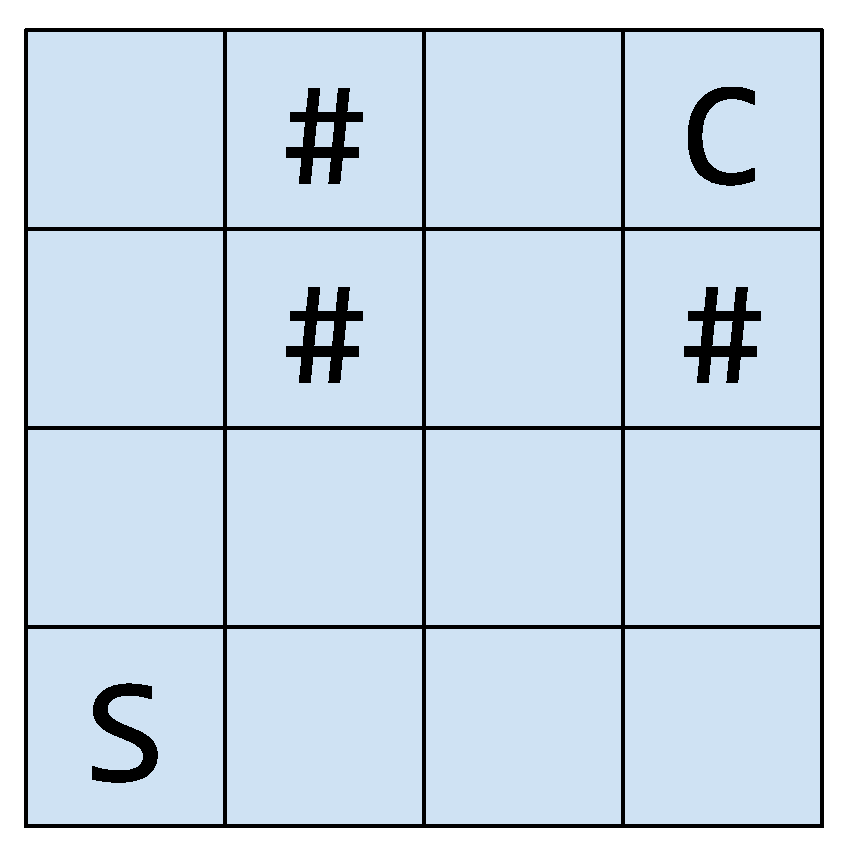
\includegraphics[width=4cm]{portals-example}
        \end{center}
    }

    \Scoring

    \begin{description}[leftmargin=0pt]
        \item[Dalinė užduotis Nr. 1 (? taškų):]
            $1 \le R \le 10, 1 \le C \le 10$.
        \item[Dalinė užduotis Nr. 2 (? taškų):]
            $1 \le R \le 50, 1 \le C \le 50$.
        \item[Dalinė užduotis Nr. 3 (? taškų):]
            $1 \le R \le 200, 1 \le C \le 200$.
            Kiekvienas atviras langelis turi bent vieną jam gretimą sienos bloką.
        \item[Dalinė užduotis Nr. 4 (? taškų):]
            $1 \le R \le 200, 1 \le C \le 200$.
        \item[Dalinė užduotis Nr. 5 (? taškų):]
            $1 \le R \le 1\ 000, 1 \le C \le 1\ 000$.
    \end{description}

    \Constraints

    \begin{description}
        \item[Laiko limitas:] 1 s.
        \item[Atminties limitas:]  MB.
    \end{description}
\end{document}
